% This is samplepaper.tex, a sample chapter demonstrating the
% LLNCS macro package for Springer Computer Science proceedings;
% Version 2.21 of 2022/01/12
%
\documentclass[runningheads]{llncs}
%
\usepackage[T1]{fontenc}
% T1 fonts will be used to generate the final print and online PDFs,
% so please use T1 fonts in your manuscript whenever possible.
% Other font encondings may result in incorrect characters.
%
\usepackage{graphicx}
% Used for displaying a sample figure. If possible, figure files should
% be included in EPS format.
%

\usepackage{hyperref}
%\usepackage{multicol}
%\usepackage{footmisc}
%\usepackage{amstext}
\usepackage{amsmath}
\usepackage{amssymb,stmaryrd}
\usepackage{mathrsfs}
\usepackage{mathtools}
%\usepackage{amsthm}
\usepackage[english]{babel}
%\usepackage[official,right]{eurosym}
\selectlanguage{english}
\hyphenation{ExecEngine DevOps}
%\newtheorem{lemma}{Lemma}


% Ampersand -----------------------------------------------------------

%\def\id#1{\text{\it #1\/}}
\newcommand{\xrightarrowdbl}[2][]{%
  \xrightarrow[#1]{#2}\mathrel{\mkern-14mu}\rightarrow
}
\newcommand{\id}[1]{\text{\it #1\/}}
\newcommand{\code}[1]{\text{\tt\small #1}}
\newcommand{\stmtText}[1]{``{\small\tt #1}''}
\newcommand{\dom}[1]{\id{dom}(#1)}
\newcommand{\cod}[1]{\id{cod}(#1)}
%\renewcommand{\int}[2]{\id{inter}(#1,#2)}
\newcommand{\relsIn}[1]{\id{relsIn}(#1)}    % maps a Term to a set of Relations
\newcommand{\popF}[1]{\id{pop}_{#1}}
\newcommand{\pop}[2]{\popF{#1}(#2)}
\newcommand{\maintain}{\mathbin{\id{maint}}}
\newcommand{\enf}{\mathbin{{\tt enforce}}}
\newcommand{\enforce}[2]{{\tt enforce}_{#1}(#2)}
\newcommand{\instance}{\mathbin{\id{inst}}}
\newcommand{\relname}[1]{\id{relname}(#1)}
\newcommand{\evt}[2]{\id{event}_{#1,#2}}
\newcommand{\src}[1]{\id{src}(#1)}
\newcommand{\tgt}[1]{\id{tgt}(#1)}
\newcommand{\viol}[2]{\violC{#1}(#2)}
\newcommand{\violC}[1]{\id{viol}_{#1}}
\newcommand{\sign}[1]{\id{sign}(#1)}
\newcommand{\powerset}[1]{\cal{P}\{#1\}}
\newcommand{\la}{\langle}
\newcommand{\ra}{\rangle}
\newcommand{\full}{V}
\newcommand{\declare}[3]{\id{#1}_{\pair{#2}{#3}}}
\newcommand{\subst}[3]{#3_{[#1\rightarrow #2]}}
\newcommand{\fullt}[2]{V_{\pair{#1}{#2}}}
\newcommand{\iden}{I}
\newcommand{\ident}[1]{I_{\id{#1}}}
\newcommand{\expr}[3]{(#1)_{#2\times #3}}
\newcommand{\pair}[2]{\langle{#1},{#2}\rangle}
\newcommand{\maprel}[2]{{\tt maprel}_{#1}({#2})}
\newcommand{\Pair}[2]{#1\times#2}
\newcommand{\pairs}[1]{\id{pairs}(#1)}
\newcommand{\triple}[3]{\langle{#1},{#2},{#3}\rangle}
\newcommand{\quadruple}[4]{\langle{#1},{#2},{#3},{#4}\rangle}
\newcommand{\atom}[1]{{\tt\small #1}}
\newcommand{\atoms}{\mathcal{A}}
\newcommand{\Atoms}{\mathbb{A}}
%\newcommand{\events}{\mathcal{E}}
%\newcommand{\Events}{\mathbb{E}}
\newcommand{\concept}[1]{{\tt\small #1}}
\newcommand{\concepts}{\mathcal{C}}
\newcommand{\Concepts}{\mathbb{C}}
\newcommand{\decls}{\mathcal{D}}  %% names of relations
\newcommand{\rels}{\mathcal{R}}   %% all relations
\newcommand{\Rels}{\mathbb{R}}   %% all relations
\newcommand{\relations}{\mathcal{M}} % representing terms. M is a subset of R.
\newcommand{\triples}{\mathcal{T}}
\newcommand{\Triples}{\mathbb{T}}
\newcommand{\Triple}[3]{#1\times#2\times#3}
\newcommand{\vertices}{N}
\newcommand{\enforces}{\mathcal{E}}
\newcommand{\rules}{\mathcal{U}}
\newcommand{\Rules}{\mathbb{U}}
\newcommand{\specrules}{\mathcal{S}}
\newcommand{\roles}{\mathcal{O}}
\newcommand{\dataset}{\mathscr{D}}
\newcommand{\Dataset}{\mathbb{D}}
\newcommand{\schema}{\mathscr{Z}}
\newcommand{\functionality}{\mathscr{F}}
\newcommand{\select}[2]{\id{select}_{#1}\{{#2}\}}
\newcommand{\migrsys}{\mathscr{M}}
\newcommand{\infsys}{\mathscr{S}}
\newcommand{\tf}[1]{\mathscr{T}(#1)}
\newcommand{\ptf}[1]{\mathscr{T}'(#1)}
\newcommand{\ti}[1]{\mathscr{I}(#1)}
\newcommand{\tic}[1]{I_{\cal C}(#1)}
\newcommand{\relAdd}{\dagger}
\newcommand{\flip}[1]{{#1}^\smallsmile} %formerly:  {#1}^\backsim
\newcommand{\kleeneplus}[1]{{#1}^+}
\newcommand{\kleenestar}[1]{{#1}^*}
\newcommand{\cmpl}[1]{\overline{#1}}
\newcommand{\rel}{\times}
\newcommand{\compose}{;}
\newcommand{\subs}{\subseteq}%{\models}
\newcommand{\fun}{\rightarrow}
\newcommand{\isa}{\preceq}
%\newcommand{\isaClos}{\sqsubseteq}
\newcommand{\typetest}{?}
\newcommand{\meet}{\sqcap}
\newcommand{\join}{\sqcup}
\newcommand{\Meet}{\bigsqcap}
\newcommand{\Moin}{\bigsqcup} % because LaTeX has already defined command \Join.
\newcommand{\order}{\ominus}
\newcommand{\anything}{\top}
\newcommand{\nothing}{\bot}
\newcommand{\rewriteto}{\rightarrow}
\newcommand{\calc}{\implies}
\newcommand{\alland}{\bigwedge}
\newcommand{\mph}[3]{#1_{#2\times #3}}
\newcommand{\mphu}[1]{#1_{\univ\times\univ}}

%-----------------------------------------
\newcommand{\kse}{\hspace*{1.7em}}
\newcommand{\ksf}{\hspace*{1em}}
\newcommand{\ksg}{\hspace*{1em}}
\newenvironment{derivation}{\begin{tabbing}\kse \= \ksf \= \ksg \= \kill}{\end{tabbing}}
%\newtheorem{definition}{Definition}
\newcommand{\term}[1]{\>\>\(#1\)\\[1ex]}
\newcommand{\rela}[2]{\>\(#1\)\>\>\{ \ #2 \ \}\\[1ex]}
\newcommand{\weg}[1]{}

\def\define#1{\label{dfn:#1}{\em #1}\index{#1}}
\def\definem#1{\label{dfnm:#1}{\em #1}\index{#1}\marge{#1}}
\newcommand{\marg}[1]{\index{#1}\marge{#1}}



\usepackage{color}
\renewcommand\UrlFont{\color{blue}\rmfamily}
%



\begin{document}
%

\title{Data Migration under a Changing Schema in Ampersand}
%
%\titlerunning{Abbreviated paper title}
% If the paper title is too long for the running head, you can set
% an abbreviated paper title here
%
\author{Sebastiaan Joosten\inst{1}\orcidID{0000-0002-6590-6220}\\ \and
Stef Joosten\inst{2,3}\orcidID{0000-0001-8308-0189}}
%
\authorrunning{S. Joosten}
% First names are abbreviated in the running head.
% If there are more than two authors, 'et al.' is used.
%
\institute{University of Minnesota, Minneapolis, USA \and Open Universiteit, Heerlen, the Netherlands\\ 
\email{stef.joosten@ou.nl} \and
Ordina NV, Nieuwegein, the Netherlands}
%
\maketitle              % typeset the header of the contribution
%
\begin{abstract}
Software generators can help increase the frequency of releases and their reliability.
They save on time spent on development and fixing human-induced mistakes by compiling a specification into a working information system.
However, many generators do not support data migrations.
Data migration is necessary when an incremental deployment changes the system's schema.
Consequently, developers tend to avoid migrations or migrate data ``by hand''.

To address this problem, this paper proposes a theory for data migrations aimed at automating the migration process.
The problem at large is how to preserve the semantics of that data under a changing schema.
This paper proposes a theory for deploying incremental change.
The theory is applicable in general but will be implemented in a software generator called Ampersand.

This paper defines a migration process that preserves the semantics of data by means of rules (constraints).
The migration process is based on assumptions and requirements that aim to capture a large class of data migrations in practice.
This paper focuses on correctness of the migration. Efficiency of the migration is outside its scope.

\keywords{Generative software \and Incremental software deployment \and Data migration \and Relation algebra \and Ampersand \and Schema change.}
\end{abstract}
%
%
%
\section{Introduction}
\label{sct:Introduction}
   In practice, information systems%
   \footnote{In the sequel, the word ``system'' refers to the phrase ``information system'', to simplify the language a little.}
   may live for many years.
   After they are built, they need to be upgraded at an ever-increasing pace to keep up with changing requirements in a dynamically evolving environment.
   Roughly half of the DevOps~\cite{BassWeberZhu15} teams that responded in a worldwide survey in 2023~\cite{HumanitecDevOps2023} are deploying software more frequently than once per day.
   Obviously, these deployments are mostly upgrades of existing systems.

   A problem occurs when an upgrade involves a change in the schema of the deployed system:
   The production data of the existing system must be migrated to fit the schema of the migrated system.
   Let us call that a "schema changing data migration" (SCDM).
   For example, adding or removing a column to a table in a relational database adds to the complexity of migrating data.
   Even worse, if a system invariant changes, some of the existing data in the system may violate the new invariant.
   For good reasons, most development teams will therefore try to avoid schema changes at all costs, fearing the risk and effort of the data migration.

   During the lifetime of a system, schema changing data migrations cannot always be avoided, however.
   It is this problem that we address in this paper.
   Data migration for other purposes has been described in the literature.
   For instance, if a data migration is done for switching to another platform or to different technology,
   e.g.~\cite{Gholami2016,Bisbal1999},
   migration engineers can and will avoid schema changes and functionality changes to avoid introducing new errors in an otherwise error-prone migration process.
   Another example, Ataei, Khan, and Walkingshaw~\cite{Ataei2021,Walkingshaw2014}, defines a migration as a variation between two data structures.
   They show how to unify databases with slight variations by preserving all variations in one comprehensive database.
   This does not cater for schema changes, however.
   Then there are SCDMs in situations without a schema or an implicit schema, e.g.~\cite{Hillenbrand2022}.
   If the schema is not available at compile time, the work will have to be done at runtime.
   This leads to versioned storage and an overhead in performance.
   This paper focuses on SCDMs in situations with an explicit schema that changes with the data migration.
   The prototypical use case for that is to frequently release upgrades of information systems in production,
   where the semantic integrity of data must be preserved across schema changes.
   Another use case is application integration for multiple dispersed data sources with explicit schemas.

   To analyze this situation, we need to define the notion of schema and how it constrains the data.
   To facilitate a formal analysis of the situation,
   we define an information system (section~\ref{sct:Information Systems}) as a pair of a schema and a dataset,
   so that we have the schema explicitly at our disposal.
   The dataset is separate, so we may consider an analysis of the schema only as a compile-time activity.
   Section~\ref{sct:Schemas} formalizes schemas as a combination of concepts, relations and rules.
   Relations are carriers of the data and concepts are needed to define them.
   Rules serve as invariants on the dataset; they constrain the data to impose semantics on the data.
   For experimental validation we use the language Ampersand~\cite{JoostenRAMiCS2017,Joosten-JLAMP2018}
   because its syntax and semantics correspond directly to these definitions.
   It has a notion of rule, which implements the invariants on the dataset.
   In this way, prototypes built in Ampersand have helped to refine the theory.

   In practice, data migrations typically follow Extract-Transform-Load (ETL) patterns~\cite{Theodorou2017},
   for which many tools are available.
   However, invariants that change yield extra work for software engineers to write the transform code,
   for which ETL tools typically provide little support.
   If automation can improve that, the frequency of SCDM's might well increase,
   and downtime for the sake of migration will become less acceptable.
   So, our research aims for zero-downtime as perceived by end-users.
   Another practical problem is that of data quality.
   Migrations typically suffer from a backlog of deteriorated data, incurring work to clean up data.
   Some of that must be done before the migration; some can wait till after the migration.
   We can define part of the data quality as satisfying semantic constraints.
   E.g. the constraint that the combination of street name, house number, postal code, and city occurs in
   a registration of valid addresses can be checked automatically.
   We can actually use invariants to help find and correct data pollution.
   We cannot use always use invariants, however.
   An example is when a person has deliberately specified a false name, without violating any of the existing invariants.

   To make the case for zero-downtime, we must distinguish between three types of constraint:
\begin{enumerate}
\item Transactional invariant\\
   A \define{transactional invariant} is a constraint is always true in a system.
   This is the classical database transaction; it may be violated temporarily, but the outside world will never notice.
   Thus, the zero-downtime requirement holds in the eyes of an end user.
\item Business invariant\\
   A \define{business invariant} is a constraint that that can be violated temporarily until the computer restores it.
   Example: All purchase orders are reflected on an order sheet, but different representations of the order sheet may be out of sync.
   On my smartphone, I see 7 purchase orders, but in my ERP system I see 6.
   The inconsistency arises because the back end application is still working on the consistency of the two.
   As a user, I must trust that the two will eventually be consistent.
   In this paper, we assume that this delay can be kept short enough to be negligible for users,
   so that the zero-downtime requirement is satisfied in their perception.
\item Business constraint\\
   A \define{business constraint} is a constraint that can be violated temporarily until a user restores it.
   Example: ``An authorized manager has to sign every purchase order.''
   We consider business constraints not to be invariants because users can violate them temporarily.
   This delay is definitely noticable for users.
   To satisfy the zero-downtime requirement, the system must be up and running to let users restore business constraints.
\end{enumerate}
   

Summarizing, the following requirements apply to SCDM'S
\begin{enumerate}
\item users must experience zero-downtime.
   Delays caused by transactional invariants or business invariants are not considered as downtime.
\item users must be able to fix business constraints, so they can be used
\item 
\end{enumerate}

   We can also use invariants to signal data pollution and make the migration system fix that.
   For that purpose we need to compute violations of invariants, so that we can restore them.
   The most important use of invariants, however, is to ensure that the migration system preserves the semantics of the data as much as possible.
   That prevents operational disruptions in the business caused by mistakes during the migration.


------------
oud

   This paper proposes a theory for data migrations that is meant to be implemented in a software generator called Ampersand.
   It aims at automating data migrations, so incremental changes can be done more reliably and faster.
   This contributes to a more agile software development process.
   We believe that users will experience a more organic evolution of the system because increments are smaller, occur more frequently and more reliably.
      
   We have not found any literature on schema changing data migrations.
   Examples like these have convinced the authors to define a new method for data migration that is specifically meant for systems in production that are
   deployed in increments.
   
   The contribution of this paper is to derive a migration schema from two artifacts: an existing system
   (which has its own schema and data set) and the specification of a desired system (which has a different schema and will ``import'' relevant parts of the existing data).   
   Our theory is based on the following assumptions and requirements:
\begin{itemize}
   \item {\em incremental deployment}\\The data migration is meant to deploy a software increment in production.
   \item {\em data pollution}\\The existing data set may be polluted, but it satisfies its schema.
   \item {\em human intervention}\\The data migration may require human interaction, which may take time.
   %\item {\em semantic continuity}\\the meaning of data must be preserved.
   \item {\em zero-downtime}\\The business continues during the migration without interruption.
   \item {\em generative software development}\\A compiler exists to generate a system from a given schema.
\end{itemize}
   This paper focuses on the correctness of the migration.
   Efficiency of the migration is beyond the scope.

\section{Analysis}
\label{sct:Analysis}
\subsection{Information Systems}
   This section defines information systems, so we can formally define the migration procedure from one system to another.

   The purpose of an information system is to store and disclose data in a way that is meaningful to its users.
   Multiple users, working from different locations and on different moments, constitute what we will loosely call ``the business''.
   The data in the system constitutes the collective memory of the business,
   which relies on the semantics of the data to draw the right conclusions and carry out their tasks.
   %This paper uses semantic constraints to represent this meaning.
   
   Actors (both users and computers) are changing the data in a system continually.
   The state of the system is represented by a data set, typically represented in a persistent store or database.
   Events that the system detects may cause the state to change.
\begin{figure}[bht]
   \begin{center}
     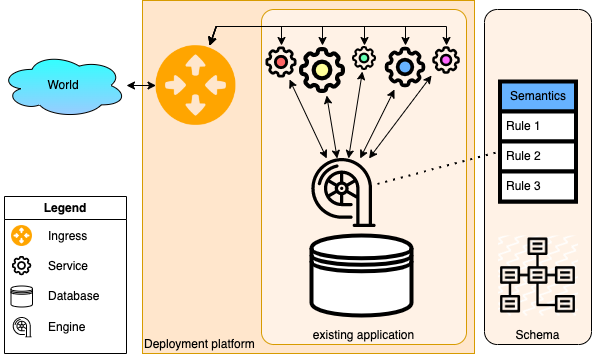
\includegraphics[scale=.45]{figures/datamigration-Pre-migration.png}
   \end{center}
\caption{Anatomy of an information system}
\label{fig:pre-migration}
\end{figure}
   To keep our theory technology independent, data sets are assumed to contain triples.
   This makes our theory valid for any kind of database that triples can represent,
   including SQL databases, object-oriented databases, graph databases, triple stores, and other no-SQL databases.
   An important aspect of the system's semantics are the constraints, sometimes known as invariants or integrity rules.
   %The purpose of these rules is to keep all constraints satisfied.

   Like most software generators, Ampersand is a compiler that generates information systems from a script.
   Ampersand uses a form of heterogeneous relation algebra,
   which works with relations in a way similar to Alloy~\cite{Alloy2006}.
   A system is then described by a set of rules (aka constraint / invariant), which the system keeps satisfied.
   So all constraints are explicitly available as rules in the Ampersand code.

   This, and the absence of imperative code in an Ampersand script, makes Ampersand a suitable platform on which to implement the theory.
   It also allows us to be explicit about ``preserving the meaning as much as possible''.
   An Ampersand script contains just enough information to generate a complete system,
   which means that a classical database schema (i.e.\ data structure plus constraints) can be extracted from the Ampersand script.

\subsection{Data Migrations}
   Data migration occurs when a desired system replaces an existing one,
   while preserving the meaning of the present data as much as possible~\cite{Spivak2012}.
   %Just copying the set of data from the existing system to the desired system is obviously wrong if the schemas of both systems differ.
   %
   In practice, data migrations are done by deploying the desired system and the existing system side-by-side,
   while transferring data in a controlled fashion, as shown in Figure~\ref{fig:migration phase}.
\begin{figure}[bht]
   \begin{center}
     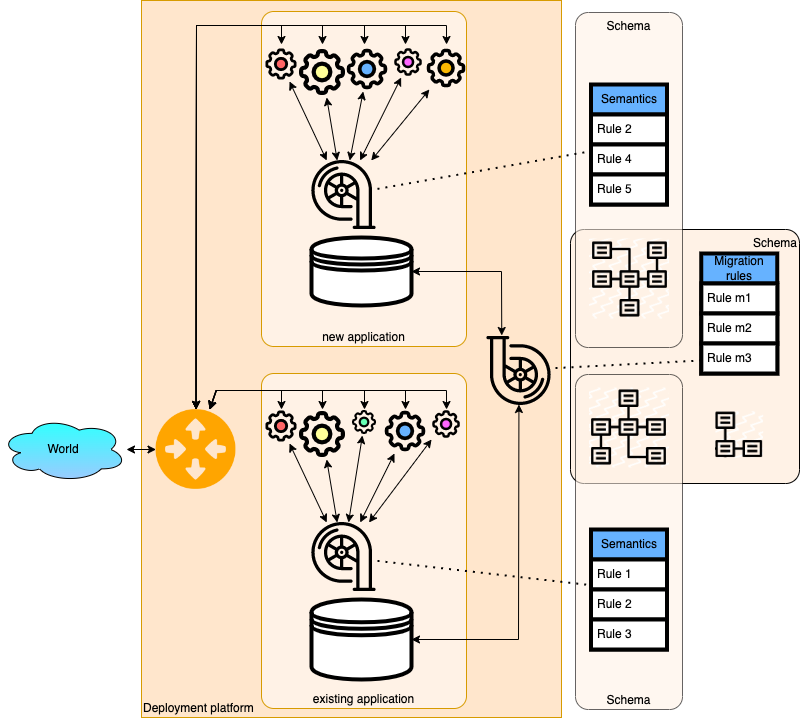
\includegraphics[scale=.35]{figures/datamigration-Migration-phase.png}
   \end{center}
\caption{Migration phase}
\label{fig:migration phase}
\end{figure}
   To automate the migration as much as possible,
   we also deploy a migration system,
   which has its own schema to specify the migration itself.
   The migration system comprises the schemas of both the existing system and the desired system,
   to implement the copying of data.
   To fully automate every data migration is unrealistic.
   A migration engineer can minimize manual work by minimizing the size of the increments,
   but she cannot eliminate it completely.
   Data pollution, new business rules, or known issues in the existing system
   may occasionally require the migration engineer to tailor the migration script to specific needs.

   A data migration has the following distinct moments\footnote{Completion can also be done gradually, but that is outside the scope of this paper.}:
\begin{enumerate}
   \item the moment of transition (the MoT), after which users experience changed functionality;
   \item the moment of completion (the MoC), after which the migration engineer removes the migration system and the old system, including its data.
\end{enumerate}

   Before the migration, the existing system satisfies its invariants (by definition).
   When the migration system compiles correctly, it satisfies its own invariants,
   so it can be deployed in production.
   That is the MoT.
   The task of the migration system is to satisfy the invariants of the desired system
   so that it can be deployed in production.
   For some of these invariants, enforcement rules can satisfy them automatically.
   There may be invariants, however, that require human interaction to resolve.
   Once all invariants of the desired system are satisfied, the migration is ready for the MoC.
   So, the schema of the migration system must contain the rules to satisfy all invariants of the desired system.

   During the migration phase, transactions in the existing system are allowed because the migration engine will transport them to the desired system.
   However, after the MoT there must be no new changes in the existing system,
   to allow the system to finish transactions while the desired system is up and running.
   
\begin{figure}[bht]
   \begin{center}
     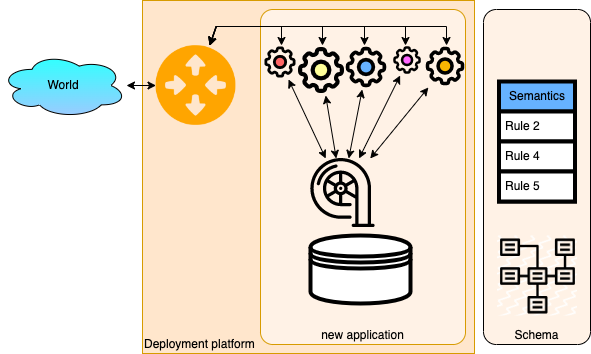
\includegraphics[scale=.35]{figures/datamigration-Post-migration.png}
   \end{center}
\caption{The system after the data migration}
\label{fig:post-migration}
\end{figure}

   The following section introduces the definitions required to migrate data from one system to another.

\section{Terminology}
\label{sct:Terminology}
   An {\em information system} is a combination of data set, schema, and functionality.
   For the purpose of this paper, functionality captured in user interfaces are ignored because it does not impact the migration.
   Section~\ref{sct:Data sets} desribes data sets. Schemas are treated in section~\ref{sct:Schemas}.
   Then section~\ref{sct:Information Systems} defines information systems.

\subsection{Data sets}
\label{sct:Data sets}
   A data set $\dataset$ describes a set of structured data, which is typically stored persistently in a database of some kind.
   The notation $\dataset_{\infsys}$ refers to the data set of a particular system $\infsys$.
   The purpose of a data set is to describe the data of a system at one point in time. 
   Before defining data sets, let us first define the constituent notions of atom, concept, relation, and triple.
   
   Atoms serve as data elements.
   %Atoms are values without internal structure of interest, meant to represent atomic data elements (e.g. dates, strings, numbers, etc.) in a database.
   %From a business perspective, atoms represent concrete items of the world,
   %such as \atom{Peter}, \atom{1}, or \atom{the king of France}.
   %By convention throughout the remainder of this paper, variables $a$, $b$, and $c$ represent \emph{atoms}.
   All atoms are taken from an infinite set called $\Atoms$.
   %
   Concepts are names that group atoms of the same type.
   All concepts are taken from an infinite set $\Concepts$.
   %$\Concepts$ and $\Atoms$ are disjoint.
   For example, a developer might choose to classify \atom{Peter} and \atom{Melissa} as \concept{Person},
   and \atom{074238991} as a \concept{TelephoneNumber}.
   In this example, \concept{Person} and \concept{TelephoneNumber} are concepts.
   Moreover, \atom{Peter}, \atom{Melissa} and \atom{074238991} are atoms.
   In the sequel, variables $A$, $B$, $C$, $D$ will represent concepts, and variables $a$, $b$, and $c$ represent \emph{atoms}.
   %
   The relation $\instance:\Pair{\Atoms}{\Concepts}$ relates atoms to concepts.
   The term $a\instance C$ means that atom $a$ is an \emph{instance} of concept $C$.
   %This relation is used in the type system, in which $\instance$ assigns one or more concepts to every atom in the data set.
   %Since $\instance$ is a relation and every relation is a set of pairs,
   %set operators $\cup$, $\cap$, and $-$ can be used on $\instance$.

   Relations serve to organize and store data, to allow a developer to represent facts.
   In this paper, variables $r$, $s$, and $d$ represent relations\footnote{Some readers might like to read `relation symbol' where we write `relation'.}.
   All relations are taken from an infinite set $\Rels$.
   $\Rels$ is disjoint from $\Concepts$ and $\Atoms$.
   Every relation $r$ has a name, a source concept, and a target concept.
   The notation $r=\declare{n}{A}{B}$ denotes that relation $r$ has name $n$, source concept $A$, and target concept $B$.
   The part $\pair{A}{B}$ is called the {\em signature} of the relation.
   
   Triples serve to represent data.
   A triple %\footnote{Please note that this paper uses the word {\em triple} in a more restricted way than in natural language.}
   is an element of $\Triple{\Atoms}{\Rels}{\Atoms}$.
   For example, $\triple{\text{\atom{Peter}}}{\declare{\id{phone}}{\tt Person}{\tt TelephoneNumber}}{\text{\atom{074238991}}}$ is a triple.
   
   \begin{definition}[Data set]
   A data set $\dataset$ is a tuple $\pair{\triples}{\instance}$ with finite $\triples \subseteq {\Triple{\Atoms}{\Rels}{\Atoms}}$ and $\instance \subseteq  {\Pair{\Atoms}{\Concepts}}$ that satisfies:
\begin{eqnarray}
   \triple{a}{\declare{n}{A}{B}}{b}\in\triples&\Rightarrow&a\instance A\ \wedge\ b\instance B
   \label{eqn:wellTypedEdge}
\end{eqnarray}
\end{definition}
   Looking at the example,
   equation~\ref{eqn:wellTypedEdge} says that \atom{Peter} is an instance of {\tt Person} and \atom{074238991} is an instance of {\tt TelephoneNumber}.
   In practice, users can say that the Person Peter has telephone number 074238991.
   So, the ``thing'' that \atom{Peter} refers to (which is Peter) has \atom{074238991} as a telephone number.
   The notations $\triples_{\dataset}$ and $\instance_{\dataset}$ are used to disambiguate $\triples$ and $\instance$ when necessary.
   To save writing in the sequel, the notation $a\ r\ b$ means that $\triple{a}{r}{b}\in\triples$.

   A relation $r$ can serve as a container of pairs,
   as defined by the function $\popF{r}:\Dataset\rightarrow\powerset{\Pair{\Atoms}{\Atoms}}$.
   It defines a set of pairs, also known as the population of $r$:
\begin{equation}
   \pop{r}{\dataset}\ =\ \{ \pair{a}{b}\mid\ \triple{a}{r}{b}\in\triples_{\dataset}\}
\label{eqn:pop-rel}
\end{equation}
%   Equation~\ref{eqn:wellTypedEdge} implies that for every data set $\dataset$:
%\[\pair{a}{b}\in\pop{\declare{n}{A}{B}}{\dataset}\ \Rightarrow\ a\instance_{\dataset}A\ \wedge\ b\instance_{\dataset}B\]
%   For a developer, this means that the type of an atom depends only on the relation in which it resides; not on the actual population of the database.
%
   We overload the notation $\popF{}$ so we can use it on concepts $\popF{C}:\Dataset\rightarrow\powerset{\Atoms}$
   and expressions.
\begin{align}
   \pop{C}{\dataset}&= \{ x\mid\ x\ \instance_{\dataset}\ C\}
\label{eqn:pop-concept}\\
   \pop{x-y}{\dataset}&= \pop{x}{\dataset} - \pop{y}{\dataset}
\label{eqn:pop-expr}
\end{align}

\subsection{Schemas}
\label{sct:Schemas}
   Schemas serve to capture the semantics of a system~\cite{Spivak2012}.
   We consider a schema to represent the static part of a system, defining concepts, relations, and rules.
   A software engineer defines a schema on design time, so that semantic checks can be implemented at compile time.

   We describe a schema $\schema$ via a tuple $\quadruple{\concepts}{\rels}{\rules}{\enforces}$,
   in which $\concepts\subseteq \Concepts$ is a finite set of concepts,
   $\rels\subseteq \Rels$ is a finite set of relations,
   $\rules\subseteq \Triple{(\Dataset \to \powerset{\Pair{\Atoms}{\Atoms}})}{\Concepts}{\Concepts}$ is a finite set of rules,
   and $\enforces\subseteq \Pair{\Rels}{\left(\Dataset \to \powerset{\Pair{\Atoms}{\Atoms}}\right)}$ is a finite set of enforcement rules.
   
   Each rule in a schema serves to constrain the data set at runtime, to ensure its semantic integrity.
   Every rule is an element of an infinite set called $\Rules$.
   In this paper, variables $u$ and $v$ represent rules.
   A rule $u$ in the schema is a triple $\triple{\violC{u}}{A}{B}$ such that $\viol{u}{\dataset}$ represents any violations to $u$ in data set $\dataset$.
   In Ampersand, rules are well-typed, just like relations:
   Every violation $\pair{a}{b}$ of a rule $\triple{\violC{u}}{A}{B}$ must satisfy $a\instance A$ and $b\instance B$.
   % For every data set $\dataset$, the set $\viol{u}{\dataset}$ is a subset of $\pop{A}{\dataset}\times\pop{B}{\dataset}$.
   If there are no violations, that is: $\viol{u}{\dataset} = \emptyset{}$, then we say that $u$ is satisfied.
   
   For a different kind of constraint, the system is told what to do in order to fix it.
   Such constraints are called enforcement rules.
   We use just one type of enforcement rule\footnote{Ampersand has several types of enforcement rules.} in this work.
   Its syntax in Ampersand is as follows:
\begin{align}
      \text{\tt ENFORCE}\ r\ \text{\tt >:}\ \id{term}\label{enforce ins}
\end{align}

   Adding an enforcement rule to the script of a system specifies a function $\violC{u} : \Dataset \to \powerset{\Pair{\Atoms}{\Atoms}}$
   with $\viol{u}{\dataset} = \pop{\id{term} - r}{\dataset}$.
   The system ensures that the rule is satisfied by adding a triple $\triple{x}{r}{y}$ for each $\pair{x}{y} \in \viol{u}{\dataset}$.
   Thus the system maintains $\pop{r}{\dataset} \supseteq \pop{\id{term}}{\dataset}$ as an invariant.
   
   Formally, enforcement rules are pairs with $u$ a function and $r$ a relation, written $r \mapsfrom t$ or equivalently $r \mapsfrom \lambda \dataset.~ t(\dataset)$.
   The set of enforcement rules in a schema is $\enforces$.
   
   \begin{definition}[Schema]
   A schema is a tuple $\quadruple{\concepts}{\rels}{\rules}{\enforces}$ that satisfies:
\begin{align}
   \declare{n}{A}{B}\in\rels&~\Rightarrow~ A\in\concepts\,\wedge\, B\in\concepts
   \label{eqn:relationsIntroduceConcepts}\\
   \triple{\violC{u}}{A}{B}\in\rules&~\Rightarrow~A\in\concepts\,\wedge\, B\in\concepts\label{eqn:rule-has-type}\\
   \triple{\violC{u}}{A}{B}\in\rules&~\Rightarrow~\forall\dataset.\ \viol{u}{\dataset}\subseteq\Pair{\pop{A}{\dataset}}{\pop{B}{\dataset}}\label{eqn:rule-well-typed}\\
   (\declare{n}{A}{B}\mapsfrom t)\in\mathcal\enforces&~\Rightarrow~ \declare{n}{A}{B}\in \rels\label{eqn:enforcement-has-type}\\
   (\declare{n}{A}{B}\mapsfrom t)\in\mathcal\enforces&~\Rightarrow~\forall\dataset.\ \pop{t}{\dataset}\subseteq\Pair{\pop{A}{\dataset}}{\pop{B}{\dataset}}\label{eqn:enforcement-well-typed}
\end{align}
   \end{definition}
   Requirement~\ref{eqn:relationsIntroduceConcepts} ensures that concepts mentioned in a relation are defined in the schema.
   This is also known as static typing, which has well established advantages for the software engineering process~\cite{HanenbergKRTS14,Petersen2014}.
   Requirements~\ref{eqn:rule-has-type} and~\ref{eqn:rule-well-typed} ensure that violations in a rule correspond to the type of that rule. 
   Requirements~\ref{eqn:enforcement-has-type} and~\ref{eqn:enforcement-well-typed} ensure the same for enforcement rules. 
   The type system of Ampersand~\cite{vdWoude2011} ensures that every system it generates satisfies requirements~\ref{eqn:relationsIntroduceConcepts} thru~\ref{eqn:enforcement-well-typed}.
   When clarity is needed, we write $\concepts_{\schema}$, $\rels_{\schema}$, $\rules_{\schema}$, and $\enforces_{\schema}$
   for $\concepts$, $\rels$, $\rules$, and $\enforces$ corresponding to $\schema = \quadruple{\concepts}{\rels}{\rules}{\enforces}$.

\subsection{Information Systems}
\label{sct:Information Systems}
   Let us now define the notion of an information system.
\begin{definition}[information system]
\label{def:information system}
\item An information system $\infsys$ is a tuple $\pair{\dataset}{\schema}$, in which
\begin{itemize}
   \item $\dataset=\pair{\triples}{\instance}$ is a data set (satisfies equation~\ref{eqn:wellTypedEdge}), we write $\triples_\infsys = \triples$ and $\instance_\infsys = \instance$;
   \item $\schema=\quadruple{\concepts}{\rels}{\rules}{\enforces}$ is a schema (satisfies equation~\ref{eqn:relationsIntroduceConcepts} thru~\ref{eqn:enforcement-well-typed}), we write $\concepts_\infsys = \concepts$, $\rels_\infsys = \rels$, $\rules_\infsys=\rules$, and $\enforces_\infsys=\enforces$;
   \item All rules and enforcement rules are satisfied:
   \begin{align}
   \forall u\in\rules&.~\viol{u}{\dataset}=\emptyset\\
   \forall (r\mapsfrom t)\in\enforces&.~\viol{u}{\dataset} - \pop{r}{\dataset}=\emptyset
   \label{eqn:satisfaction}
   \end{align}
   \item Triples in the data set have their relation mentioned in the schema:
   \begin{eqnarray}
   \triple{a}{\declare{n}{A}{B}}{b}\in\triples&\Rightarrow&\declare{n}{A}{B}\in\rels
   \label{eqn:define R}
   \end{eqnarray}
\end{itemize}
\end{definition}
   % A \define{role} is a name that identifies a group of users.
   % It serves as a placeholder for a person or a machine (i.e. an actor) that works with the data set (i.e. create, read, update, or delete triples).
   % The purpose of a role is to mention an individual user (human) or an automated actor (bot) without knowing who that user is.

   As the system responds to events, it changes its data set, while the schema remains the same.
   In this paper, it suffices to define an event as a pair of systems for which the schema stays constant.
   Events are categorized by the part of the data set that changes.
   
\begin{definition}[Event]
   Let $R \subseteq \Rels$ and $I \subseteq \Rels$ be sets of relations,
   and let $\infsys=\pair{\schema}{\dataset}$ and  $\infsys'=\pair{\schema}{\dataset'}$ be information systems,
   then $\infsys\xrightarrow[I]{R} \infsys'$ is an event if and only if:
   \begin{align}
      \triple{a}{r}{b}\in\triples_{\dataset}-\triples_{\dataset'}&\Rightarrow\ r\in R
   \label{eqn:eventUnchanged}\\
      \triple{a}{r}{b}\in\triples_{\dataset'}-\triples_{\dataset}&\Rightarrow\ r\in(R \cup I)
   \label{eqn:eventInsert}
   \end{align}
   % was:
   % \begin{align}
   %    \triples_{\dataset} - (\Triple{\Atoms}{(R \cup I)}{\Atoms}) &= \triples_{\dataset'} - (\Triple{\Atoms}{(R \cup I)}{\Atoms})
   % \label{eqn:eventUnchanged}\\
   %    \triples_{\dataset} - (\Triple{\Atoms}{R}{\Atoms}) &\subseteq \triples_{\dataset'} - (\Triple{\Atoms}{R}{\Atoms})
   % \label{eqn:eventInsert}
   % \end{align}
   We say that event $\infsys\xrightarrow[I]{R} \infsys'$ brings the system $\infsys$ to $\infsys'$ inserting pairs in relations from $I$ and deleting pairs in relations from $R$.
\end{definition}
   
   Equation~\ref{eqn:eventUnchanged} and~\ref{eqn:eventInsert} state that the triples of those for relations in $I$ or $R$ are the only ones that can be changed, and that only triples in $R$ can be removed.
   %If $I$ or $R$ is the empty set, we omit it from the arrow, so $\infsys \xrightarrow{R} \infsys'$ is a notation for $\infsys \xrightarrow[\emptyset]{R} \infsys'$.
   
\begin{definition}[Inserting event]
   We write $\infsys \xrightarrowdbl[I]{R} \infsys'$ to state that some triple was inserted whose relation was in $I$, that is:
   $t \in \triples_{\dataset'} \cap (\Triple{\Atoms}{I}{\Atoms})$ and $t \not\in \triples_{\dataset}$ for some triple $t$.
\end{definition}
   
   We use inserting events to model the effect of enforcement rules.
%   If $R$ is a set of relations that covers those that occur in the rule, then changes to an system $\infsys$ can be described by the event $\infsys \xrightarrow[\{r\}]{R} \infsys'$.

\subsection{Example}
\label{sct:Example existing IS}
   Having defined information systems in mathematical terms, let us discuss a small example.
   It is written in the language Ampersand to make it more appealing to read.
   Let us first define a data set of just a handful of triples and three relations.
\begin{verbatim}
RELATION takes[Student*Course] =
[ ("Peter", "Management")
; ("Susan", "Business IT")
; ("John", "Business IT")
]
\end{verbatim}
   This declaration introduces a relation with the name \verb#takes#,
   source concept \verb#Student#, and
   target concept \verb#Course#.
   The informal meaning of this relation is that it states which students are taking which courses.

   The example system also has a second relation that states which modules are part of which course.
\begin{verbatim}
RELATION isPartOf[Module*Course] =
[ ("Finance", "Management")
; ("Business Rules", "Business IT")
; ("Business Analytics", "Business IT")
; ("IT-Governance", "Management")
]
\end{verbatim}
   The third relation states which students are enrolled for which module.
   It is left without population for now.
\begin{verbatim}
RELATION isEnrolledFor[Student*Module]
\end{verbatim}

   A rule, {\tt EnrollRule} completes the script.
   It states that a student can enroll for any module that is part of a course she takes.
   % In Ampersand, which is a syntactically sugared form of relation algebra~\cite{JoostenRAMiCS2017},
   % each rule has a name and each rule has a role to maintain its invariance:
\begin{verbatim}
RULE EnrollRule: isEnrolledFor |- takes;isPartOf~
\end{verbatim}
   The Ampersand compiler defines $\viol{\tt EnrollRule}{\dataset}$ as
\begin{equation}
   \pop{\tt isEnrolledFor}{\dataset}-\{\pair{s}{m} \mid\exists c.~s\ \text{\tt takes}\ c\ \wedge\ m\ \text{\tt isPartOf}\ c\}
\end{equation}
   This rule is satisfied if $\viol{\tt EnrollRule}{\dataset}=\emptyset$, which means that
\begin{equation}
   \begin{array}{l}
   \forall \pair{s}{m}\in\pop{\tt isEnrolledFor}{\dataset}.~ \exists c\in\text{\tt Course}~.\\
   s\ \text{\tt isEnrolledFor}\ m\ \rightarrow\ s\ \text{\tt takes}\ c\ \wedge\ m\ \text{\tt isPartOf}\ c
   \end{array}
\label{eqn:example isEnrolledFor}
\end{equation}
   In this example, relation $\declare{\tt isEnrolledFor}{\tt Student}{\tt Module}$ is empty, so rule {\tt EnrollRule} is satisfied.

   Now let us check the requirements to verify that this example defines an information system.
   % Requirement~\ref{eqn:specialization} is satisfied because this example contains no specialization.
   The Ampersand compiler generates a data set $\dataset$, which contains a set of triples and a relation $\instance$.
   It defines the set of triples $\triples$ as:
\[\begin{array}[t]{l}
   \triple{\text{\tt "Peter"}}{\declare{\text{\tt takes}}{\text{\tt Student}}{\text{\tt Course}}}{\text{\tt "Management"}}\\
   \triple{\text{\tt "Susan"}}{\declare{\text{\tt takes}}{\text{\tt Student}}{\text{\tt Course}}}{\text{\tt "Business IT"}}\\
   \triple{\text{\tt "John"}}{\declare{\text{\tt takes}}{\text{\tt Student}}{\text{\tt Course}}}{\text{\tt "Business IT"}}\\
   \triple{\text{\tt "Finance"}}{\declare{\text{\tt isPartOf}}{\text{\tt Module}}{\text{\tt Course}}}{\text{\tt "Management"}}\\
   \triple{\text{\tt "Business Rules"}}{\declare{\text{\tt isPartOf}}{\text{\tt Module}}{\text{\tt Course}}}{\text{\tt "Business IT"}}\\
   \triple{\text{\tt "Business Analytics"}}{\declare{\text{\tt isPartOf}}{\text{\tt Module}}{\text{\tt Course}}}{\text{\tt "Business IT"}}\\
   \triple{\text{\tt "IT-Governance"}}{\declare{\text{\tt isPartOf}}{\text{\tt Module}}{\text{\tt Course}}}{\text{\tt "Management"}}
\end{array}\]
The relation $\instance$ contains the pairs:
\[\begin{array}{l}
   \pair{\text{\tt "Finance"}}{\tt Module}\\
   \pair{\text{\tt "Business Rules"}}{\tt Module}\\
   \pair{\text{\tt "Business Analytics"}}{\tt Module}\\
   \pair{\text{\tt "IT-Governance"}}{\tt Module}\\
   \pair{\text{\tt "Management"}}{\tt Course}\\
   \pair{\text{\tt "Business IT"}}{\tt Course}\\
   \pair{\text{\tt "Peter"}}{\tt Student}\\
   \pair{\text{\tt "Susan"}}{\tt Student}\\
   \pair{\text{\tt "John"}}{\tt Student}
\end{array}\]
   The pair $\pair{\triples}{\instance}$ satisfies requirement~\ref{eqn:wellTypedEdge} so this is a data set $\dataset$ as introduced in section~\ref{sct:Data sets}.

   The Ampersand compiler generates a schema $\schema$, which contains concepts, a specialization relation, relations, and rules.
   It defines the sets of concepts, relations, and rules to obtain a schema $\schema$:
\[\begin{array}{rcl}
   \concepts&=&\{ {\tt Module}, {\tt Course}, {\tt Student}\}\\
   \rels&=&\{\begin{array}[t]{@{}l@{}}
               \declare{\tt takes}{\tt Student}{\tt Course},\\
               \declare{\tt isPartOf}{\tt Module}{\tt Course},\\
               \declare{\tt isEnrolledFor}{\tt Student}{\tt Module}\}
             \end{array}\\
   \rules&=&\{ {\tt EnrollRule}\}\\
   \enforces&=&\emptyset
  \end{array}
\]
   % The user has defined no specializations.
   % This means that $\isa$ equals the identity relation on $\concepts$ and requirements~\ref{eqn:isasIntroduceConcepts} and~\ref{eqn:isasPartialOrder} are satisfied.
   % The script defines the set of rules $\rules$ to contain just one rule: \verb-EnrollRule-.
   % The (nonempty) data set satisfies this rule, which meets requirement~\ref{eqn:consistentRules}.
   So, the schema $\schema=\quadruple{\concepts}{\rels}{\rules}{\enforces}$ satisfies all requirements from section~\ref{sct:Schemas}.

   Now let us check the definition of information system.
   Requirement~\ref{eqn:satisfaction} is satisfied because the only rule, {\tt EnrollRule} is satisfied.
   This satisfies definition~\ref{def:information system}, which establishes that $\infsys$ is an information system.
   % The set of roles is empty and so is the relation $\maintain$.
   % This meets all requirements for $\infsys=\triple{\dataset}{\schema}{\roles}{\maintain}$ from definition~\ref{def:information system}.
   % This concludes the argument that $\infsys$ is an information system.

\section{Generating a Migration Script}
   A migration script takes care of two things: copying data and ensuring that the migration system is a proper information system.
   Sections~\ref{sec:loading} and~\ref{sec:violations on invariants} illustrate how this works by example, using the Ampersand syntax.
   Then, section~\ref{General migration script} defines what this means in general terms.

\subsection{Loading Data}\label{sec:loading}
   Let us study how to migrate data from $\dataset$ to $\dataset'$.
   It would be tempting to state that a relation from the example system, say {\tt isPartOf}, could be copied by the following code fragment%
\footnote{The prefix {\tt old.} refers to concepts, relations, and rules from the existing system (section~\ref{sct:Example existing IS}).
The prefix {\tt new.} refers to items from the desired system.}:
\begin{verbatim}
   ENFORCE new.isPartOf >: old.isPartOf
\end{verbatim}
   The relation {\tt old.isPartOf} resides in the existing system and will not change after the MoT.
   
   This means, however, that anything in {\tt old.isPartOf} cannot be deleted from {\tt new.isPartOf}.
   This is undesirable because it prevents us from changing data in the migration system.
   The desired behavior is that all pairs in {\tt old.isPartOf} are copied to {\tt new.isPartOf} when the system is first initialized, but that {\tt new.isPartOf} can be changed freely after that.
   An extra relation (\ref{extraRelation}) achieves this behavior by remembering which pairs have been copied:
\begin{eqnarray}
   &&\verb#RELATION copied_isPartOf[Student*Course]#\label{extraRelation}\\
   &&\verb#ENFORCE new.isPartOf >: old.isPartOf - copied_isPartOf#\label{difference}\\
   &&\verb#ENFORCE copied_isPartOf >: new.isPartOf#\label{fill copies with new.isPartOf}
\end{eqnarray}
   
   Let us look what happens at runtime.
   Initially, when {\tt copied\_isPartOf} is still empty, the difference between {\tt old.isPartOf} and {\tt copied\_isPartOf} equals {\tt old.isPartOf}.
   So, {\tt new.isPartOf} will contain the pairs of {\tt old.isPartOf} by rule~\ref*{difference}.
   Then, the engine inserts the same pairs into {\tt copied\_isPartOf} because of rule~\ref*{fill copies with new.isPartOf}.
   After this, triples with the relation {\tt new.isPartOf} can be inserted and deleted freely.
   Once all triples have been copied, {\tt copied\_isPartOf} will contain all pairs of {\tt old.isPartOf} and rule~\ref*{difference} will no longer insert any triples in {\tt new.isPartOf}.
   So, this rule can be removed after the copying has taken place.
   Consequently, declarations~\ref{extraRelation} thru~\ref{fill copies with new.isPartOf} can be removed from the migration script at the MoC.

\subsection{Dealing with violations on invariants}\label{sec:violations on invariants}
   Suppose the script for the desired system adds an invariant that is not present in the existing system:
   
\begin{verbatim}
   RELATION isPartOf[Module*Course] [UNI]
\end{verbatim}
   
   The \verb=UNI= annotation requires that each \verb=Module= is part of at most one \verb=Course=.
   The violations are given by:
\begin{eqnarray}
   \viol{\tt UNI}{\dataset} = \{\pair{x}{y} \mid x \neq y \wedge \exists z.~ \pair{z}{x}, \pair{z}{y}\in\pop{\tt isPartOf}{\dataset} \}
\end{eqnarray}
   In Ampersand, the term that gives these violations is: \verb=isPartOf~;isPartOf - I=.
   
   While the \verb=UNI= requirement holds for the population in the original script, that population may have changed.
   Therefore, we must assume that we cannot expect that \verb=new.isPartOf= satisfies the \verb=UNI= requirement in the desired system.
   The migration system allows for this by simply not requiring that they hold at the MoT.
   A challenge lies in ensuring that they do hold at the MoC, and that users that help the migration forward can achieve a state in which all requirements hold.
   
   Two extra relations are used: one to track the violations that occur in the original data (\ref{violRelation}), and one to track the violations that have been fixed (\ref{fixedRelation}) which prevents them from recurring.
\begin{align}
   &\text{\tt RELATION viols\_UNI[Course*Course]}\label{violRelation}\\
   &\text{\tt RELATION fixed\_UNI[Course*Course]}\label{fixedRelation}\\
   &\text{\tt ENFORCE viols\_UNI >: old.isPartOf\textasciitilde;old.isPartOf - I}\label{fill viols}\\
   &\text{\tt ENFORCE fixed\_UNI >: viols\_UNI - (new.isPartOf\textasciitilde;new.isPartOf - I)}\label{fill fixed}\\
   &\begin{aligned}
   \text{\tt RULE isPartOf\_UNI: new.isPartOf\textasciitilde;new.isPartOf}\\
   \quad\text{\tt |- I \textbackslash/ (viols\_UNI - fixed\_UNI)}
   \end{aligned}\label{rule uni}
\end{align}
   
   We again look at what happens at runtime:
   Enforcement rule~\ref{fill viols} adds all violations present in the old system to {\tt viols\_UNI}.
   Until the MoT, rule~\ref{fill fixed} does nothing, since {\tt viols\_UNI} equals $\viol{\tt UNI}{\dataset}$.
   At that point, rule~\ref{rule uni} is satisfied, since the right-hand side of equation~\ref{rule uni} is empty.
   As violations are fixed, rule~\ref{fill fixed} records this by adding to {\tt fixed\_UNI}.
   This way, previously fixed errors cannot recur.
   Once {\tt viols\_UNI} is equal to {\tt fixed\_UNI}, the \verb=UNI= requirement holds and the system is ready for the MoC in regard to this rule.
   
   We also wish to alert users with the role `migration helper' to violations that need to be fixed.
   For the original \verb=UNI= requirement, this means specifying:
   
\begin{align}
   \begin{aligned}
   \text{\tt RULE isPartOf\_UNI\_warn: new.isPartOf\textasciitilde;new.isPartOf |- I}\\
   \quad\text{\tt ROLE MigrationHelper}
   \end{aligned}\label{warnings}
\end{align}
   
   Despite the syntax, Line~{\ref{warnings}} is not a rule of the generated system in the formal sense:
   By assigning a role, the responsibility of maintaining the rule no longer lies with the system.
   Instead, users with the migration helper role can see the violations and act on it as they see fit, so the only effect of Line~{\ref{warnings}} is that such users will be shown its violations.

\subsection{General migration script}\label{General migration script}
   So far, we illustrated how to do migration by giving two concrete examples.
   This section generalizes those ideas by giving a general approach for generating a migration script.
   
   Let $\pair{\dataset}{\schema}$ be the existing system, and let ${\schema'}$ be the schema of the desired system.
   Then we define the migration systems $\migrsys$ and the events as follows:
\begin{enumerate}
\item We take a disjoint union of the relations, defining $\overleftarrow~$ and $\overrightarrow~$ as (overloaded) notation to generate new names, keeping the dataset of the old system and the rules of the new system:
   \begin{align}
   \overleftarrow{\declare{n}{x}{y}}&=\declare{(\id{old}.n)}{x}{y}&\overleftarrow{X} &= \{\overleftarrow{x}\mid x\in X\}\\
   \overrightarrow{\declare{n}{x}{y}}&=\declare{(\id{new}.n)}{x}{y}& \overrightarrow{X} &= \{\overrightarrow{x}\mid x\in X\}\\
   \triples_\migrsys &= \{\triple{a}{\overleftarrow{r}}{b} \mid \triple{a}{r}{b}\in\triples_\dataset\}&
   \instance_\migrsys &= \instance_\dataset\\
   \rels_\theenumi &= \overleftarrow\rels_{\schema} \cup \overrightarrow\rels_{\schema'}
   %&\rules_\theenumi &= \rules_\schema
   \end{align}
\item We create enforcement rules to copy equal relations, corresponding to equation~\ref{extraRelation} through~\ref{fill copies with new.isPartOf} in Section~\ref{sec:loading}:
   \begin{align}
   \widetilde{\declare{n}{x}{y}} &= \declare{(\id{copied}.n)}{x}{y}\\
   \rels_\theenumi &= \{\widetilde{r}\mid r \in \rels_\schema \cap \rels_{\schema'}\}\\
   \enforces_\theenumi &= \{\overrightarrow{r}\mapsfrom \popF{\overleftarrow{r} - \widetilde{r}} \mid \widetilde{r} \in \rels_2\} \cup \{\widetilde{r}\mapsfrom \popF{\overrightarrow{r}} \mid \widetilde{r} \in \rels_2\}
   \end{align}
\item For each rule, we generate two helper relations, {\tt viols} and {\tt fixed}. Note that Rule~\ref{warnings} only influences the user interface and therefore is not modeled here. This corresponds to equation~\ref{violRelation} through~\ref{rule uni}.
   \begin{align}
   \overleftarrow{\dataset'} &= \pair{\{\triple{x}{{r}}{y}\mid \triple{x}{\overleftarrow{r}}{y} \in \triples_{\dataset'}\}}{\instance_{\dataset'}}\\
   \overrightarrow{\dataset'} &= \pair{\{\triple{a}{{r}}{b} \mid \triple{a}{\overrightarrow{r}}{b}\in\triples_\dataset\}}{\instance_{\dataset'}} \\
   \rels_\theenumi &= \{{\tt viols}_u\mid u \in \rules_{\schema'}\} \cup \{{\tt fixed}_u\mid u \in \rules_{\schema'}\}\\
   \rules_\migrsys &= \{\lambda {\dataset'}.~ \viol{u}{\overrightarrow{\dataset'}} - \pop{{\tt viols}_u - {\tt fixed}_u}{\dataset'} \mid u\in\rules_{\schema'}\}\label{eqn:migrsysrules}\\
   \enforces_{\theenumi} &=\{{\tt viols}_u \mapsfrom \lambda \dataset'.~ \viol{u}{\overleftarrow{\dataset'}}\} \cup
    \{{\tt fixed}_u \mapsfrom \lambda \dataset'.~ {\tt viols}_u - \viol{u}{\overrightarrow{\dataset'}}\}\label{eqn:enforceForRules}
   \end{align}
\item Combining the above into a single migration system:
   \begin{align}
   \concepts_\migrsys &= \concepts_\dataset \cup  \concepts_{\dataset'}\\
   \rels_\migrsys &= \rels_1\cup\rels_2\cup \rels_3\\
   %\rules_\migrsys &= \rules_1\cup \rules_3\\
   \enforces_\migrsys &= \enforces_1\cup\enforces_2\cup\enforces_3
   \end{align}
\end{enumerate}
   
\subsection{Validation}
   We first observe that $\migrsys = \pair{\pair{\triples_\migrsys}{\instance_\migrsys}}{\quadruple{\concepts_\migrsys}{\rels_\migrsys}{\rules_\migrsys}{\enforces_\migrsys}}$ is a system after application of the enforcement rules:
   the only rules are those introduced in equation~\ref{eqn:migrsysrules}, and enforcement rules from equation~\ref{eqn:enforceForRules} ensure that $\popF{{\tt viols}_u} = u$ initially, while $\popF{{\tt fixed}_u}$ is empty.
   Hence, the MoT can happen after the enforcement rules have been applied, giving us $\migrsys'$.
   The event $\migrsys \xrightarrow[\rels_2 \cup \rels_3]{\overrightarrow\rels_{\schema'}}\migrsys'$ represents the MoT.
   
   The MoC is reached for dataset $\dataset'$ whenever $\pop{{\tt viols}_u - {\tt fixed}_u}{\dataset'}=\emptyset$ for all rules.
   This should happen after a finite number of inserting events: let $I = \{{\tt fixed}_u \mid u\in\rules_{\schema'}\}$ be the relations that keep track of which violations have been fixed, then there is no infinite chain of systems $\migrsys' = \migrsys_0, \migrsys_1,\ldots$ such that $\migrsys_i\xrightarrowdbl[I]{\overrightarrow\rels_{\schema'}}\migrsys_{i+1}$.
   This shows that when users get rid of violations, there is real progress: they can only do this a finite number of times.
   Next we ask ourselves: does this mean we always reach the MoC?
   
   Suppose there is a system in which all violations have been fixed, that is, suppose there is a $\migrsys^C$ such that $\pop{{\tt fixed}_u}{\dataset_{\migrsys^C}}=\pop{{\tt viols}_u}{\dataset_{\migrsys^C}}$ and $\migrsys'\xrightarrow[I]{\overrightarrow\rels_{\schema'}} \migrsys^C$.
   In that case, after any steps done by users (both those with and without the migration helper role), we can reach it, that is: for any $\migrsys_i$, $\migrsys'\xrightarrow[I]{\overrightarrow\rels_{\schema'}} \migrsys_i$ implies $\migrsys_i\xrightarrow[I]{\overrightarrow\rels_{\schema'}} \migrsys^C$.
   This implies that if the MoC is initially reachable through $\xrightarrow[I]{\overrightarrow\rels_{\schema'}}$ events, then it will remain reachable.
   So is the MoC initially reachable?
   
   For this last question, we need to add a condition:
   There needs to be a system that has the desired schema $\schema'$.
   If rules in $\schema'$ are such that they cannot all be satisfied, regardless of the dataset, no such system exists and we have no hope of reaching it.
   We assume that the rules of $\schema'$ are intended to prevent data pollution, such that a dataset $\dataset'$ describing the `real world' would be one that satisfies them.
   So let $\pair{\dataset'}{\schema'}$ be a system, then we can get to it through our migration system.
   To show this, we construct a migration system $\migrsys^C$ satisfying $\pop{{\tt fixed}_u}{\dataset_{\migrsys^C}}=\pop{{\tt viols}_u}{\dataset_{\migrsys^C}}$ and $\migrsys'\xrightarrow[I]{\overrightarrow\rels_{\schema'}} \migrsys^C$.
   We can do so by simply stating its triples, since the schema is determined by $\migrsys'$:
   
\begin{align}
   \begin{aligned}
   \triples_{\migrsys^C} &= \triples_\migrsys 
   \cup  \{\triple{a}{{\tt viols}_u}{b} \mid \pair{a}{b}\in \viol{u}{\dataset}, u\in \rules_{\schema'} \} \\
   &\cup \{\triple{a}{{\tt fixed}_u}{b} \mid \pair{a}{b}\in \viol{u}{\dataset}, u\in \rules_{\schema'} \}
   \cup \{\triple{a}{\overrightarrow{r}}{b} \mid \triple{a}{r}{b}\in\triples_{\dataset'}\}   
   \end{aligned}
\end{align}
   
   Collectively, this shows that the MoC is and remains reachable after a finite number of inserting events by users in the migration helper role.
   
\section{Conclusions}

   In this paper, we describe the data migration as going from an existing system to a desired one, where the schema changes.
   As Ampersand generates information systems, creating a new system can be a small task, allowing for incremental deployment of new features.
   We describe the parts of a system that have an effect on data pollution.
   We assume that the existing system does not violate any constraints of its schema, but address other forms of data pollution:
   constraints that are not in the schema but are in the desired schema are initially relaxed such that the business can start using the migration system, after which this form of data pollution needs to be addressed by human intervention.
   We propose a method for doing migration such that only a finite amount of human intervention is needed.
   Our method allows a system similar to the desired system to be used while the intervention takes place.

   Our proposed migration is certainly not the only approach one could think of.
   However, we have not come across other approaches that allow changing the schema in the presence of constraints.
   As such, we cannot compare our approach against other approaches.
   We envision that one day there will be multiple approaches for migration under a changing schema to choose from.
   For now, our next step is to implement the approach shown here into Ampersand.

   This work does not consider what to do about (user) interfaces.
   Instead, it models events by assuming that any change to the dataset can be achieved.
   In practice, such changes need to be achieved through interfaces.
   Most Ampersand systems indeed allow the users of the system to edit the dataset quite freely through the interfaces.
   However, some interfaces may require certain constraints to be satisfied, which means that interfaces of the desired system might break.
   In the spirit of the approach outlined here, we hope to generate migration interfaces that can replace any broken interfaces until the Moment of Transition.
   How to do this is future work.

%\section{Bibliography}
\bibliographystyle{splncs04}
\bibliography{doc}


\end{document}
